\documentclass[12pt]{article}
\usepackage{scrextend}
\usepackage[utf8]{inputenc}
\usepackage[polish]{babel}
\usepackage[T1]{fontenc}%polskie znaki
\usepackage[utf8]{inputenc}%polskie znaki
\usepackage{geometry}
\usepackage{float}
\usepackage{enumitem}
\usepackage{hyperref}
\usepackage{graphicx}
\usepackage{tabulary}
\usepackage{etoc}
\usepackage[normalem]{ulem} 
\renewcommand{\baselinestretch}{1.5}
\graphicspath{ {img/} }
\newgeometry{lmargin=2cm, rmargin=2cm, tmargin=2cm, bmargin=2cm}
\usepackage{tikz}
\usepackage[bf]{caption}

\begin{document}

\begin{flushright}
        Damian Koper, \textbf{241292} \\
        Łukasz Handschuh, \textbf{241402}
\end{flushright}
\vspace{1cm}
{
    \centering
    {\Huge\scshape\bfseries Inżynieria oprogramowania - Etap 1 }\\
    \vspace{0.25cm}
    \Large\textbf{Dział ewidencji ludności} \\
    \vspace{0.25cm}
    \large Wykonanie opisu biznesowego „świata rzeczywistego” projektowanego oprogramowania. Definicja wymagań funkcjonalnych i niefunkcjonalnych.\\
}

\section{Opis zasobów ludzkich}

Pracownik urzędu gminy może wprowadzić informacje dotyczące zameldowania mieszkańca. Meldunek może być wprowadzony jako meldunek stały, czasowy, przeszły. Pracownik wprowadza wiosek dostarczony przez ubiegajacego się o meldunek mieszkańca do systemu. Pracownik może zatwierdzić lub odrzucić wniosek. Zatwierdzenie prowadzi do faktycznego zarejestrowania meldunku w systemie.

Wniosek meldunkowy zawiera dane takie jak:
\begin{itemize}
    \item Dane osobowe mieszkańca
    \item Dane adresowe nowego miejsca pobytu
    \item Dane adresowe dotychczasowego miejsca pobytu
    \item Zgody i oświadczenia
    \item Dane identyfikujące wniosek (nr. wniosku)
\end{itemize}

Osoba składające wniosek nie ma dostępu do systemu. Wniosek dostarczyć można jedynie drogą papierową, osobiście, lub pocztą. Dalej wniosek przetwarzany jest przez pracowników urzędu.

\section{Przepisy, strategia firmy}

Pracownik jest odpowiedzialny za poprawne wprowadzenie wniosku oraz odpowiada materialnie za niezdogność danych. System jest dostępny tylko dla pracowników urzędu i powinien zapewniać maksymalną prostotę i dostępność na wielu platformach.

\section{Dane techniczne}
Wgląd do dostępnych danych i ich edycja jest możliwa za pośrednictwem strony internetowej ze względu na dużą dostępność na wszystkich platformach i w wielu miejscach bez potrzeby instalacji. Wszyscy pracownicy mają równożędne uprawnienia. Transmisja danych jest szyfrowana.

Dane wniosków są weryfikowane poprzez kontakt z systemem PESEL.
\section{Wymagania funkcjonalne}

\subsection{Pracownicy}
\begin{enumerate}
    \item Pracownik może zalogować się na swoje konto i z niego się wylogować.
    \item Pracownik z rolą administratora może zarządzać kontami użytkowników.
    \begin{enumerate}
        \item Administrator może stworzyć konto użytkownika.
        \item Administrator może edytować dane i jego rolę użytkownika.
        \item Administrator może usunąć konto użytkownika.
    \end{enumerate}
\end{enumerate}
\subsection{Zarządzanie wnioskami}
\begin{enumerate}
    \item Pracownik może wyświetlić dane wniosków.
    \begin{enumerate}
        \item Pracownik może wyświetlić wnioski tylko danego typu.
        \item Pracownik może wyszukać wniosek podając nr. PESEL.
    \end{enumerate}
    \item Pracownik może wprowadzić wniosek meldunkowy.
    \begin{enumerate}
        \item Pracownik może wprowadzić wniosek o typie \textit{stały} lub \textit{czasowy}.
    \end{enumerate}
    \item Pracownik może edytować dane wniosku meldunkowego.
    \begin{enumerate}
        \item Pracownik może zmienić status wniosku - zaakceptować, lub odrzucić po podaniu powodu.
        \item Zaakceptowany wniosek zmienia się w rekord meldunku.
    \end{enumerate}
    \item Wniosek, by być możliwym do zaakceptowania, musi zawierać komplet danych, które zgadzają się z danymi z systemu PESEL.
\end{enumerate}
\subsection{Zarządzanie meldunkami}
\begin{enumerate}
    \item Pracownik może wyświetlić dane meldunków.
    \begin{enumerate}
        \item Pracownik może wyświetlić dane meldunków tylko danego typu.
        \item Pracownik może wyszukać dane meldunku podając nr. PESEL.
    \end{enumerate}
    \item Pracownik może edytować dane meldunków.
    \begin{enumerate}
        \item Pracownik może zmienić status meldunku na przeszły.
    \end{enumerate}
\end{enumerate}
\section{Wymagania niefunkcjonalne}
\begin{enumerate}
    \item Wszyscy użytkownicy, którzy mają dostęp do aplikacji (posiadają indywidualne konto) mają uprawnienia do edycji danych meldunkowych.
    \item Rola administratora pozwala na zarządzanie użytkownikami i ich uprawnieniami.
    \item System rejestruje historię wszystkich zmian danych meldunkowych.
    \item Dane przesyłane pomiędzy aplikacją, a systemem PESEL są szyfrowane.
    \item W przypadku braku łączności z systemem PESEL pracownik otrzymuje ostrzeżenie o tym fakcie.
    \item Podstawowym źródłem dostępu do danych jest aplikacja internetowa.
    \item Aplikacja umożliwia dostęp do danych przez podstawowy interface konsoli.
\end{enumerate}
\newpage
\newgeometry{top=1cm,left=1cm,bottom=2cm,right=1cm}
\begin{figure}[]
    \centering
    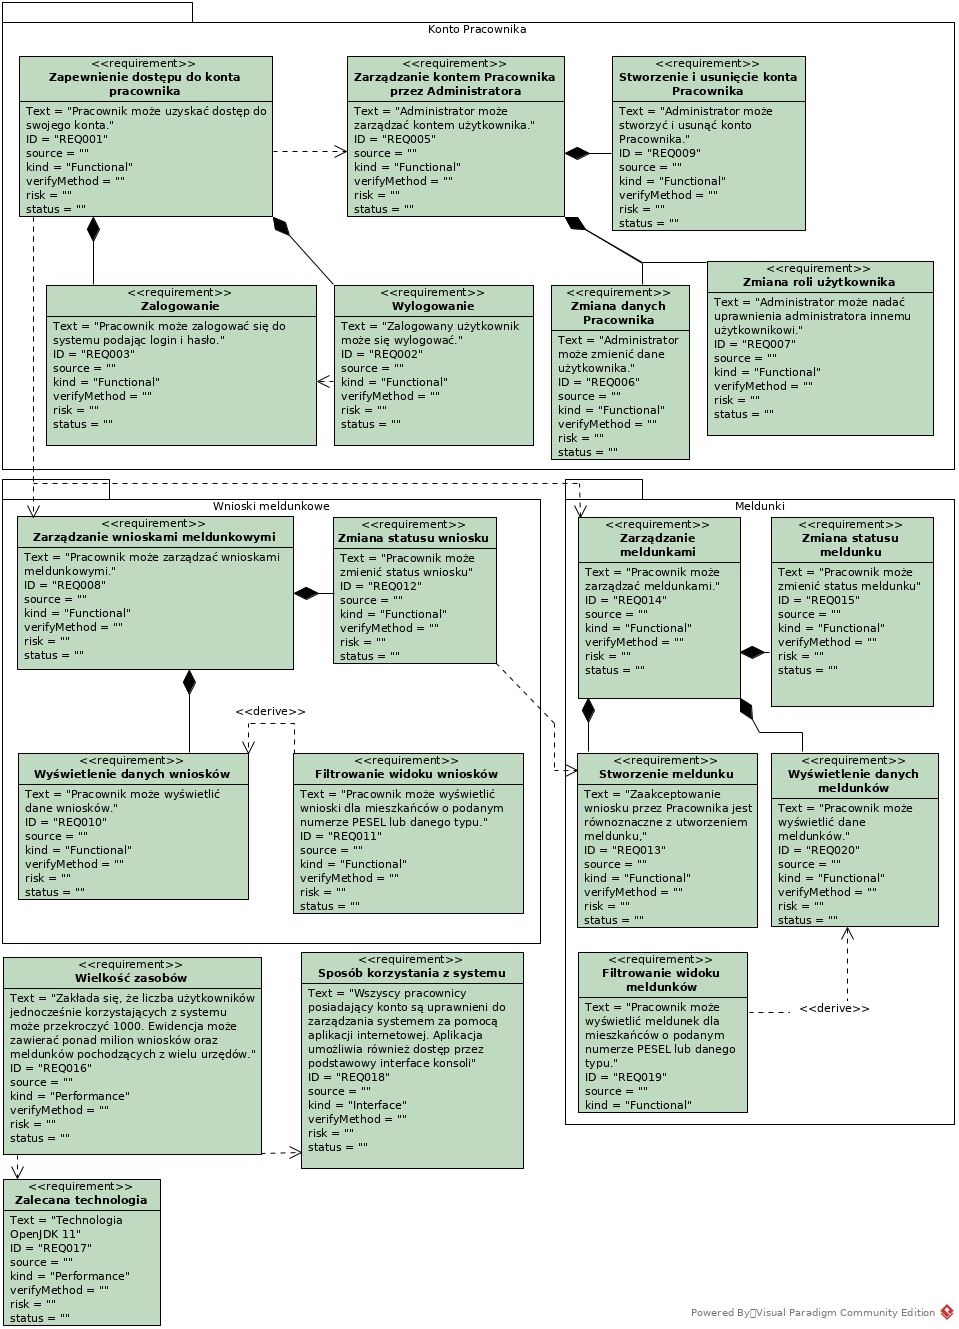
\includegraphics[
        keepaspectratio,
        width=\linewidth,
        height=\dimexpr\textheight-0\baselineskip
    ]{./../paragidm/export/PopulationRegistry_req.jpg}
    \caption{Diagram wymagań}
    \label{}
\end{figure}
\restoregeometry
\end{document}